% Standalone preview of a redrawn Figure 5.1 (the two-timescale design).
% Compile with:  pdflatex p2design_arch.tex
% To adopt it, replace the tikzpicture inside \begin{figure} in
% sections/5_multipath.tex (keep the existing \caption and \label).
%
% What changed relative to the version in the thesis:
%   * the "per-path state: ..." label sat on top of the Transport agent box and
%     ran past the figure's right edge; it is now two lines, below the feedback
%     arrow, inside the drawing area;
%   * the path boxes were narrower than the text they hold, so "path N
%     (live/dead)" overflowed on both sides; they are wider and the liveness
%     note is a second line;
%   * "target bitrate" sat on the arrow between the two agent boxes; the gap is
%     wider and the label sits above the arrow;
%   * the two reward return paths ran at nearly the same height and their labels
%     touched the dashed lines; the delivery reward now returns over the top of
%     the path column (it used to rise at x = 8.15, grazing the scorer box and
%     cutting across all three fan-out arrows) and the application reward has
%     the bottom lane to itself;
%   * \resizebox is gone. The picture is laid out at 0.86 of its natural size,
%     so the small labels stay above 6pt at \linewidth instead of being scaled
%     to whatever the width demanded.
\documentclass[border=4pt]{standalone}
\usepackage[T1]{fontenc}
\usepackage{newpxtext,newpxmath}
\usepackage{tikz}
\usetikzlibrary{arrows.meta,positioning,fit,calc,backgrounds}
\usepackage[mode=text, detect-all, binary-units=true, per-mode=symbol,
            range-phrase=\,--\,, range-units=single]{siunitx}
\usepackage{xcolor}
\definecolor{eth1}{HTML}{1F407A}
\definecolor{eth5}{HTML}{91056A}
\definecolor{eth7}{HTML}{A8322D}
\definecolor{eth10}{HTML}{82BE1E}
\begin{document}
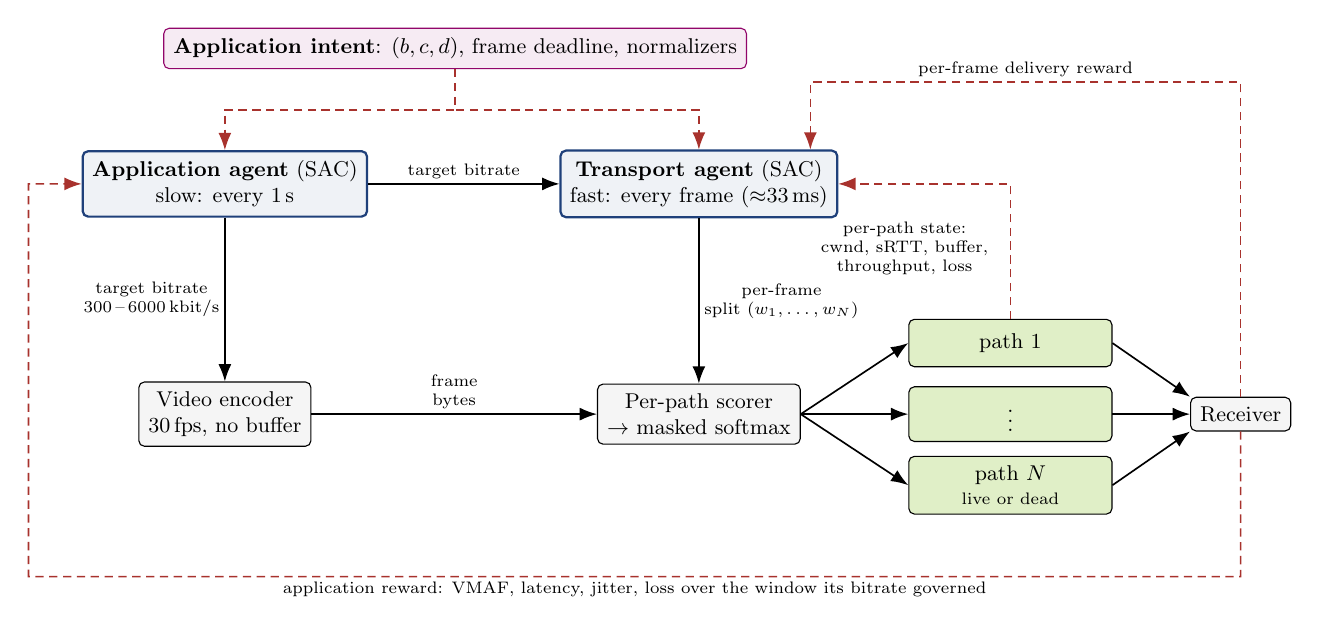
\begin{tikzpicture}[
  scale=0.86, every node/.style={transform shape}, font=\small,
  box/.style={draw, rounded corners=2pt, align=center, inner sep=4pt},
  agent/.style={box, thick, draw=eth1, fill=eth1!7},
  unit/.style={box, fill=black!4},
  pathb/.style={box, fill=eth10!25, minimum width=30mm, minimum height=7mm},
  flow/.style={-{Latex[length=2.2mm]}, semithick},
  sig/.style={-{Latex[length=2.2mm]}, semithick, densely dashed, draw=eth7},
  lbl/.style={font=\scriptsize, align=center, inner sep=2pt},
]
  % --- intent ---
  \node[box, draw=eth5, fill=eth5!8] (intent) at (3.4,5.4)
    {\textbf{Application intent}: $(b,c,d)$, frame deadline, normalizers};
  % --- agents ---
  \node[agent] (app) at (0,3.4)
    {\textbf{Application agent} (SAC)\\ slow: every \SI{1}{\second}};
  \node[agent] (tr) at (7.0,3.4)
    {\textbf{Transport agent} (SAC)\\ fast: every frame (${\approx}\SI{33}{\milli\second}$)};
  % --- data plane ---
  \node[unit] (enc) at (0,0.0) {Video encoder\\ 30\,fps, no buffer};
  \node[unit] (spl) at (7.0,0.0) {Per-path scorer\\ $\rightarrow$ masked softmax};
  \node[pathb] (p1) at (11.6,1.05) {path 1};
  \node[pathb] (p2) at (11.6,0.0) {$\vdots$};
  \node[pathb] (p3) at (11.6,-1.05) {path $N$\\[-1pt] {\scriptsize live or dead}};
  \node[unit] (rx) at (15.0,0.0) {Receiver};
  % --- intent into both agents ---
  \draw[sig] (intent.south) -- ++(0,-0.6) -| (app.north);
  \draw[sig] (intent.south) -- ++(0,-0.6) -| (tr.north);
  % --- control flow ---
  \draw[flow] (app.south) -- node[lbl, left] {target bitrate\\ \SIrange{300}{6000}{\kilo\bit\per\second}} (enc.north);
  \draw[flow] (app.east) -- node[lbl, above, pos=0.5] {target bitrate} (tr.west);
  \draw[flow] (tr.south) -- node[lbl, right] {per-frame\\ split $(w_1,\dots,w_N)$} (spl.north);
  \draw[flow] (enc.east) -- node[lbl, above] {frame\\ bytes} (spl.west);
  \draw[flow] (spl.east) -- (p1.west);
  \draw[flow] (spl.east) -- (p2.west);
  \draw[flow] (spl.east) -- (p3.west);
  \draw[flow] (p1.east) -- (rx.north west);
  \draw[flow] (p2.east) -- (rx.west);
  \draw[flow] (p3.east) -- (rx.south west);
  % --- feedback: per-path state, routed above the path column into the agent ---
  \draw[sig] (p1.north) |- (tr.east);
  \node[lbl, anchor=east] at (11.35,2.45)
    {per-path state:\\ cwnd, sRTT, buffer,\\ throughput, loss};
  % --- feedback: per-frame delivery reward, own lane above the path column ---
  % It used to run back at y = -2.1 and rise at x = 8.15, which grazed the
  % scorer box and cut across all three fan-out arrows. It now returns over the
  % top, where the only thing at that height is empty space.
  \coordinate (trtop) at ($(tr.north)!0.8!(tr.north east)$);
  \coordinate (rlane) at (15.0,4.9);
  \draw[sig] (rx.north) -- (rlane) -- node[lbl, pos=0.5, above]
    {per-frame delivery reward} (trtop |- rlane) -- (trtop);
  % --- feedback: application reward, own lane below everything ---
  \draw[sig] (rx.south) -- (15.0,-2.4) -- node[lbl, pos=0.5, below]
    {application reward: VMAF, latency, jitter, loss over the window its bitrate governed}
    (-2.9,-2.4) -- (-2.9,3.4) -- (app.west);
\end{tikzpicture}
\end{document}
